\documentclass[12pt]{article}
\usepackage{fullpage}
\usepackage{lastpage}
\usepackage{fancyhdr}
\pagestyle{fancy}

\addtolength{\topmargin}{-0.25in}
\usepackage{graphicx}	
\usepackage{array, multicol}
\usepackage{amsmath}
\usepackage{comment}
\usepackage{enumerate}
\usepackage{url}

\everymath{\displaystyle}

\fancypagestyle{plain}{
	\fancyhf{}
	\addtolength{\headheight}{2.92\baselineskip}
	\lhead{\bf MATH 2554 (Calculus I) \\
		Spring 2016 \\
		}
	\rhead{{Name:} \underline{\hspace{40ex}} \\
		\vspace{0.5pc}
		Fri 12 Feb 2016}
	\rfoot{Exam 1 p.\thepage\ (of \pageref{LastPage})}
	}
\fancyhf{}
\renewcommand{\headrulewidth}{0pt}

\title{\vspace{-8pc}
\vfill{\Huge
	\bf Exam 1: Limits (\S 2.1-3.1)} 
	}
\author{}
\date{}

\rfoot{Exam 1 p.\thepage\ (of \pageref{LastPage})}

% % % % %
\begin{document}
\maketitle
\vspace{-3pc}
\noindent{\bf Exam Instructions:} You have 50 minutes to complete this exam.  Justification is required for all problems. 

\vspace{2pc}
\noindent\textbf{Your signature below indicates that you have read this page and agree to follow the Academic Honesty Policies of the University of Arkansas.}  

\vfill
\noindent Signature: {\bf (1 pt)} \underline{\hspace{73ex}}
\begin{flushright}\Large Good luck!\end{flushright}
\begin{enumerate}

% % % % %
\newpage
\item {\bf (10 pts)} Let $f(x)=\frac{x+7}{x^4-49x^2}$.  Identify all vertical asymptotes for $f$ (or if there are none, say so and why).  Then, for each vertical asymptote $a$, find $\lim_{x\to a^+}f(x)$ and $\lim_{x\to a^-}f(x)$.	

% % % % %
\newpage
\item {\bf (10 pts)} Determine the end behavior of $f(x)=\frac{x+1}{\sqrt{9x^2+x}}$.  If there are any horizontal asymptotes then identify them.

% % % % %
\newpage
\item {\bf (3 pts ea)} Evaluate the following limits analytically:
\begin{enumerate}
	\item $\lim_{y\to 3}\frac{\sqrt{3y+16}-5}{y-3}$
	\vspace{22pc}
	
	\item $\lim_{x\to 0}(2x^{-8}+4x^3)$
	\newpage
	\item $\lim_{x\to \infty}\pi e^{-x}$
	\vspace{22pc}
	
	\item $\lim_{t\to -1}f(t)g(t)$, given that $\lim_{t\to -1}f(t)=2$ and $\lim_{t\to -1}g(t)=8$.
\end{enumerate}

% % % % %
\newpage
\item {\bf (10 pts)} 
Use the Intermediate Value Theorem to show $f(x)=4x^3-6x^2+3x-2$ must cross the line $y=10$ in the interval $(1,2)$.

% % % % %
\newpage
\item {\bf (3 pts ea)} Let $f(x)=x^2-2x+3$.  Below is a graph of $f(x)$, drawn at \url{desmos.com}.
\begin{center}
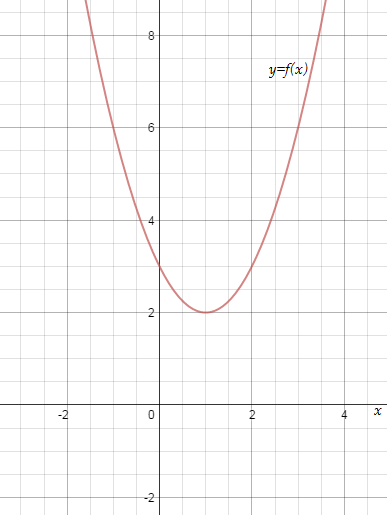
\includegraphics[scale=0.4]{exam1Parabola}
\end{center}
\begin{enumerate}
	\item Use the graph to find a number $\delta>0$ such that if $|x-1|<\delta$ then $|f(x)-2|<1$.  If no such number exists, then say so.
	\vspace{4pc}
	
	\item If, when we use smaller and smaller values $\epsilon<1$, we can always find a corresponding value $\delta>0$, as in (a), then we will have proved that 
	\[
	\qquad\qquad\qquad\qquad\qquad\qquad\lim_{x\to ?}f(x)=? \quad\text{(rewrite the limit, with the ?s filled in).}
	\]
	\vspace{2pc}
	%\item {\bf (7 pts)} For $\epsilon=\textstyle\frac{1}{4}$, find $\delta>0$ so that $|f(x)-2|<\epsilon$ whenever $0<|x-1|<\delta$.  \textit{Hint: In setting up the inequality, solve for $x-1$ instead of $x$.}
	%\vspace{12pc}
	\item For \textit{any} $\epsilon>0$, find $\delta>0$ so that $|f(x)-2|<\epsilon$ whenever $0<|x-1|<\delta$.  \textit{Hint: Your answer will be an expression with $\epsilon$s in it.} 
	\end{enumerate}  

% % % % %
\newpage
\item When computing derivatives in this problem you must use the limit definitions.  Given the function,
\[s(t)=\sqrt{5t}\]
	\begin{enumerate}
	\item {\bf (5 pts)} write the formula for the slope of the secant line joining the points $(a,s(a))$ and $(b,s(b))$;
	\vspace{14pc}
	
	\item {\bf (5 pts)} find $s'(1)$;
	\vspace{14pc}
	
	\item {\bf (3 pts)} write the equation of the line tangent to $s(t)$ at $t=1$.
	\end{enumerate}
	
% % % % %
\newpage
\item {\bf (5 pts)} Find constants $b$ and $c$ in the polynomial $p(x)=x^2+bx+c$ so that 
\[
\lim_{x\to 2}\frac{p(x)}{x-2}=6.
\]
\vspace{22pc}
% % % % %
%\newpage
\item {\bf (5 pts) } Determine the interval(s) of continuity for
\[f(x)=\frac{x+2}{x^2-4}.\]

% % % % %
\end{enumerate}
\end{document}